
%%------------------------
%% Oct 9, 2021
%% Y. Lee
%% (D) Interactive Geometry
%% 1. Geometric constructions
%% Source of this Activity: Exploring Conic Sections with The Geometer’s SketchPad © 2002 Key Curriculum Press
%%------------------------

\documentclass[11pt]{article}
\usepackage{latexsym,amssymb}%,times,mathptm}
\usepackage{amsmath}
\usepackage{amscd}
\usepackage{makeidx}
\usepackage{enumerate}
\usepackage{graphicx}

\input xypic
\baselineskip=55pt


\textwidth=6.5in
\hoffset=-0.8 in
\voffset=-0.5 in
\textheight=8.3 in


\newcommand{\mi}[1]{#1\index{#1}}
\newcommand{\llar}{-\kern-5pt-\kern-5pt\longrightarrow}



\def\ann{\mbox{\rm ann}}
\def\Ass{\mbox{\rm Ass}}


\begin{document}

\begin{center}
{\bf MAT 140 \quad Computational Tools for Mathematics and the Sciences}

\end{center}

\medskip
\noindent {Chapter:  \quad Geometry}

\smallskip

\noindent {Technology: GeoGebra}

\smallskip

\noindent {Section:  \quad \quad Composition of Isometries}

\smallskip

\noindent {Activity time: 50 minutes}


\vspace{0.2 in}


\noindent {\bf I. Preamble}

\smallskip

\noindent In this lab, you will learn how to use GeoGebra to observe the results of composing two or more isometries. Remember, {\bf an isometry} is a distance-preserving transformation between metric spaces, such as a translation, a rotation, and a reflection. The following are function notations for each of the isometries. 
	\begin{enumerate}[(a)]
	\item Translation \\ $T_{\vec{PQ}}$ 	
	\item Rotation \\ $R_{O, \theta}$
	\item Reflection \\ $M_l$ 
	\item Glide reflection (the composition of a translation with a reflection) \\ $G_{\vec{PQ}, l}$\\
	\end{enumerate}


\vspace{0.2 in}

\noindent {\bf II. Constructing a GeoGebra model}


\begin{enumerate}[(1)]
\item Use GeoGebra to translate, rotate, or reflect an object using an appropriate set of parameter(s).

	\begin{center}
	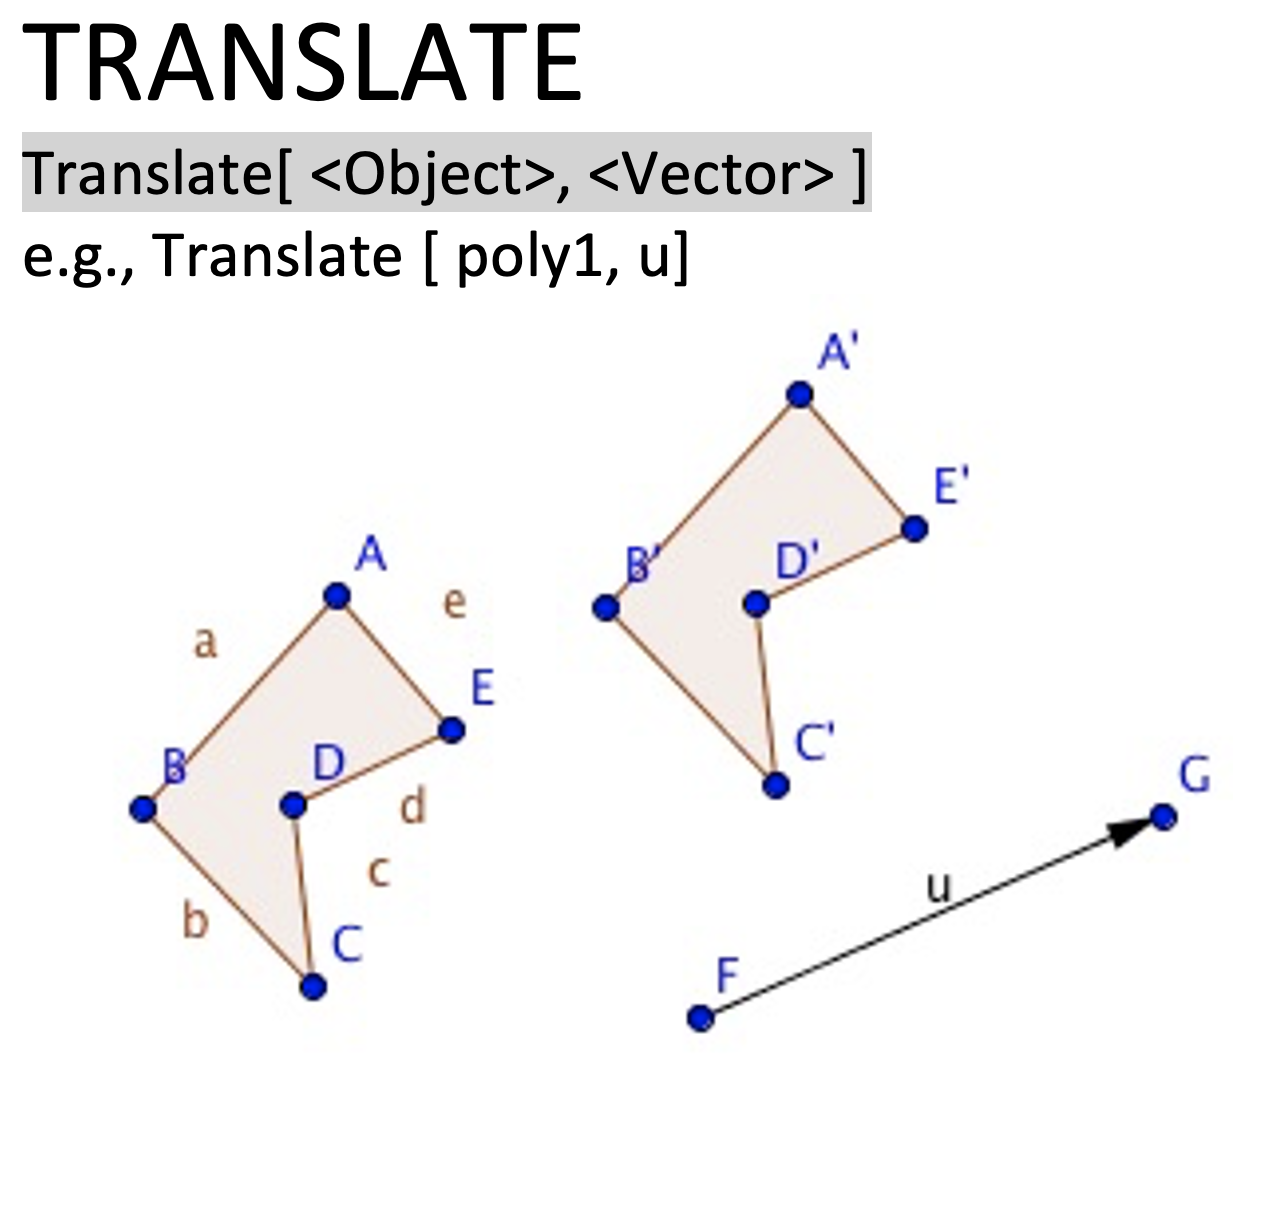
\includegraphics[height=0.27\textheight]{figure_1.png} \hspace{0.2cm} 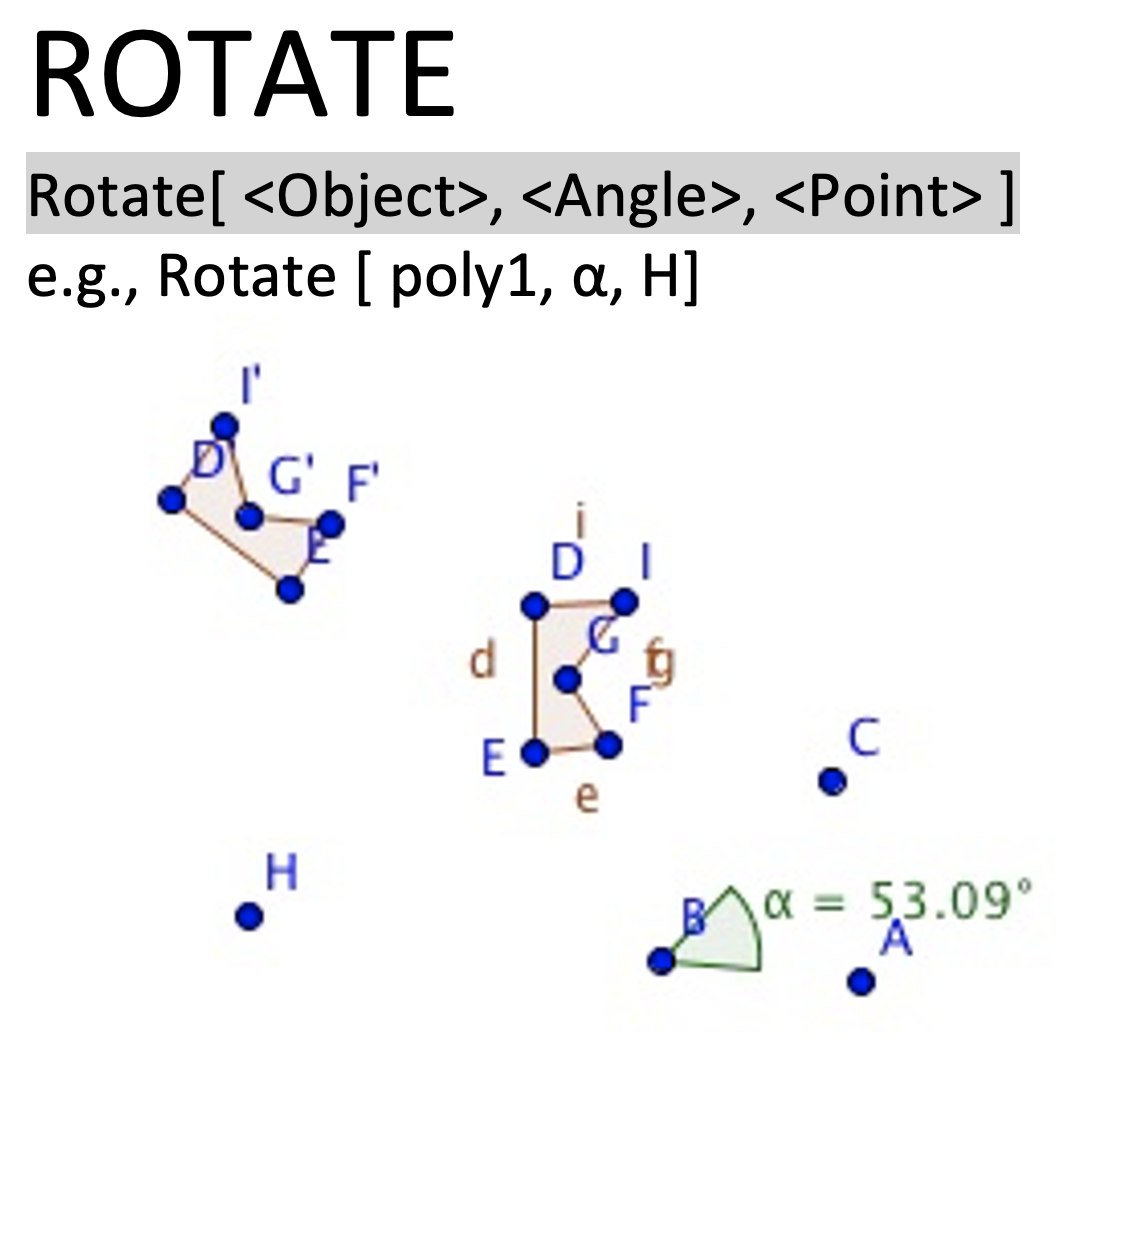
\includegraphics[width=0.25\textheight]{figure_2.png}   \hspace{0.2cm}  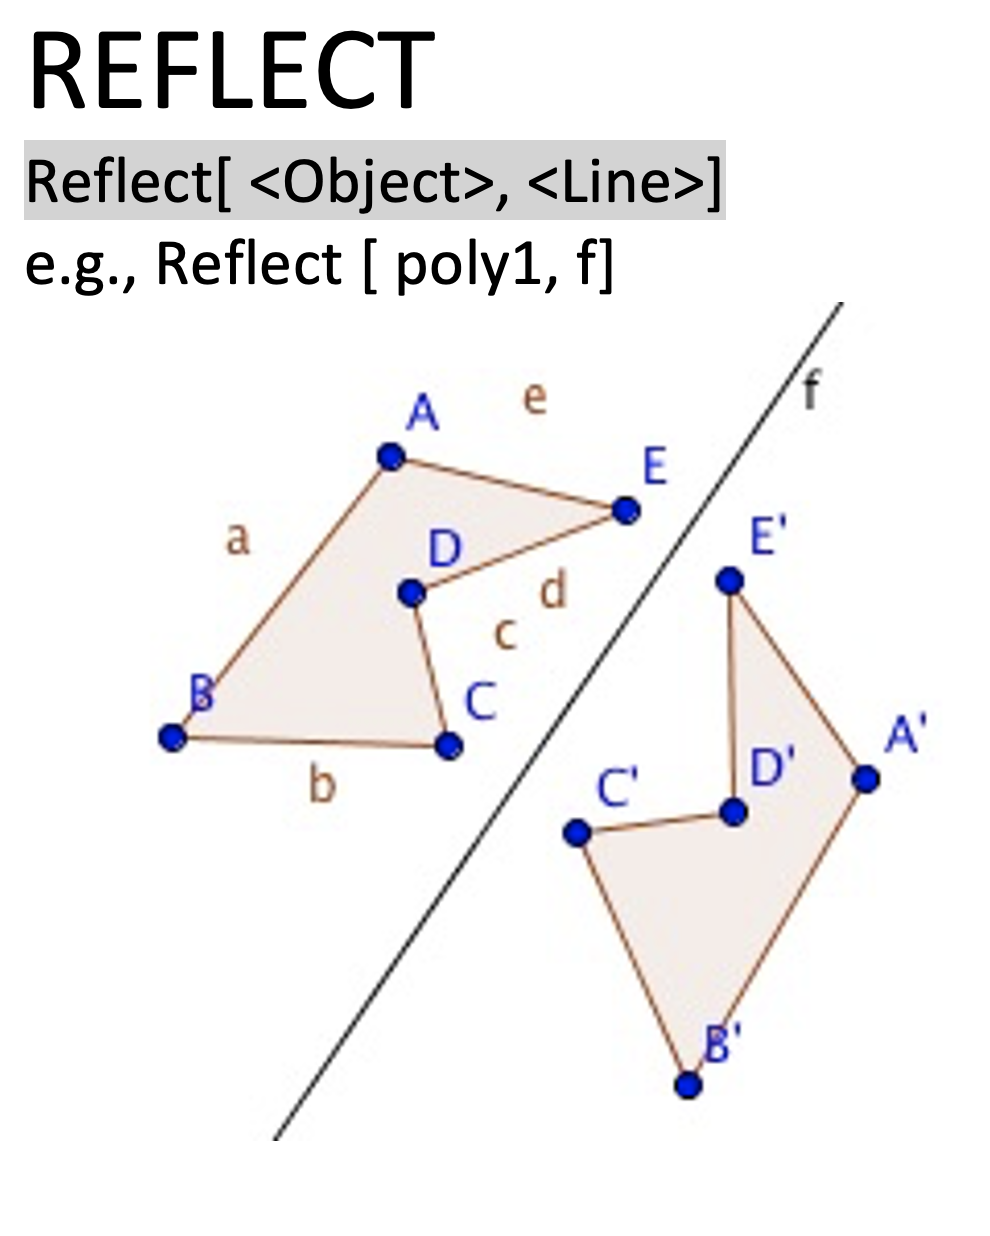
\includegraphics[width=0.25\textheight]{figure_3.png}
	\end{center}

\item {\bf The composition of two reflections with two parallel lines}: Reflect $ \bigtriangleup ABC$ through the two parallel lines $o$ and $n$ according to the following composition: $M_o \circ M_n$. Describe your results. Can you get from $ \bigtriangleup ABC$ to $ \bigtriangleup A''B''C''$ directly (that is, using only one transformation)? If so, describe the transformation and, in so doing, identify the parameters in terms of the parameters of the functions that make up the composition.  

	\begin{center}
	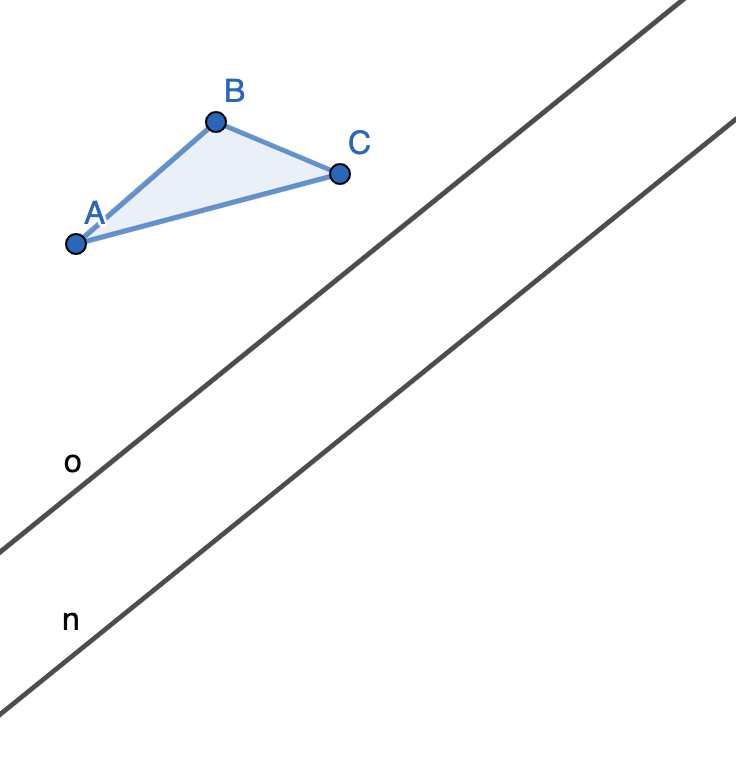
\includegraphics[height=0.45\textheight]{figure_4.png} 
	\end{center}


\pagebreak
\item {\bf The composition of two reflections with two intersecting lines}: Find the single isometry equivalent to the composition: $M_o \circ M_n$. Prove your result. How about $M_n \circ M_o$? Be sure to identify the parameters in terms of the parameters of the functions that make up the composition.  

	\begin{center}
	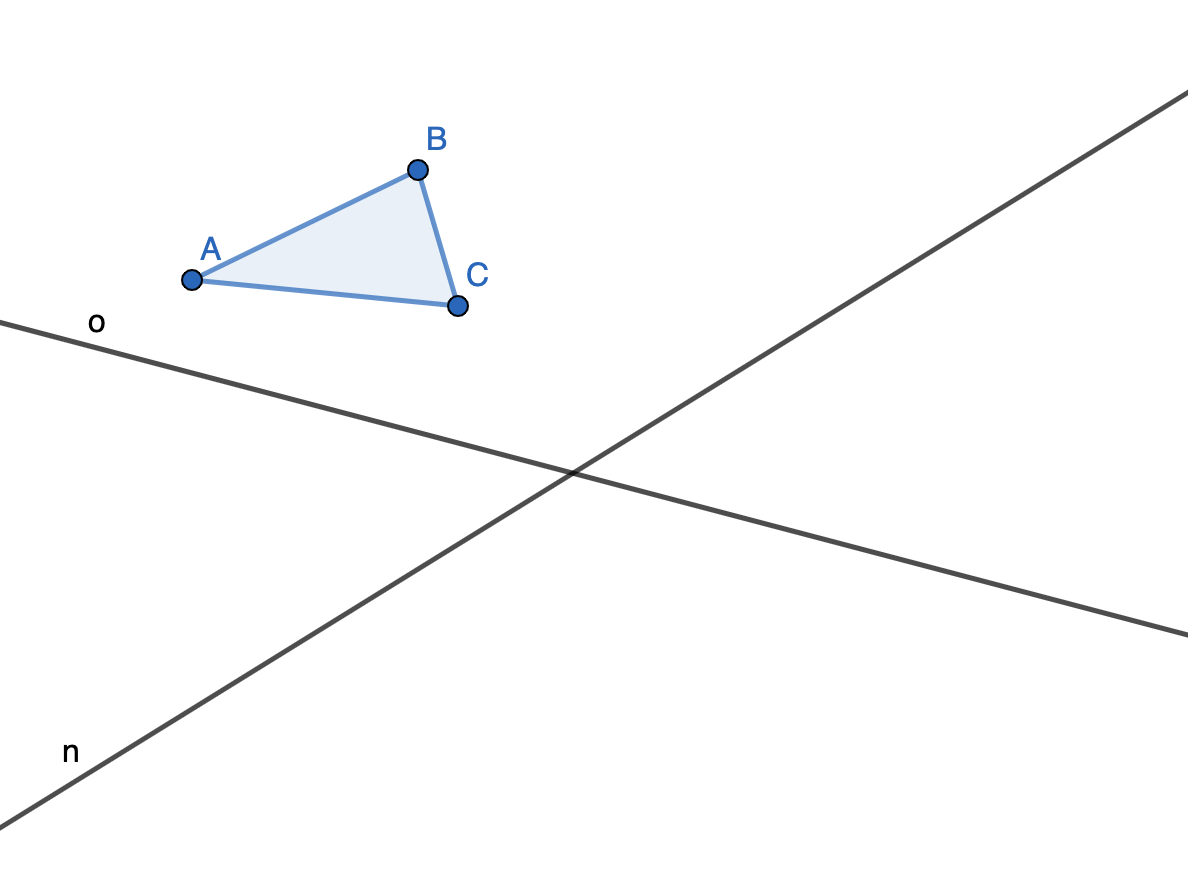
\includegraphics[height=0.45\textheight]{figure_5.png} 
	\end{center}
	
\pagebreak	
\item {\bf The composition of three reflections}: As shown in the figure below, line $p$ and $n$ are parallel and they are both perpendicular to line $o$. Identify the single isometry that is equivalent to the following composition: $M_o \circ M_n \circ M_p$. 

	\begin{center}
	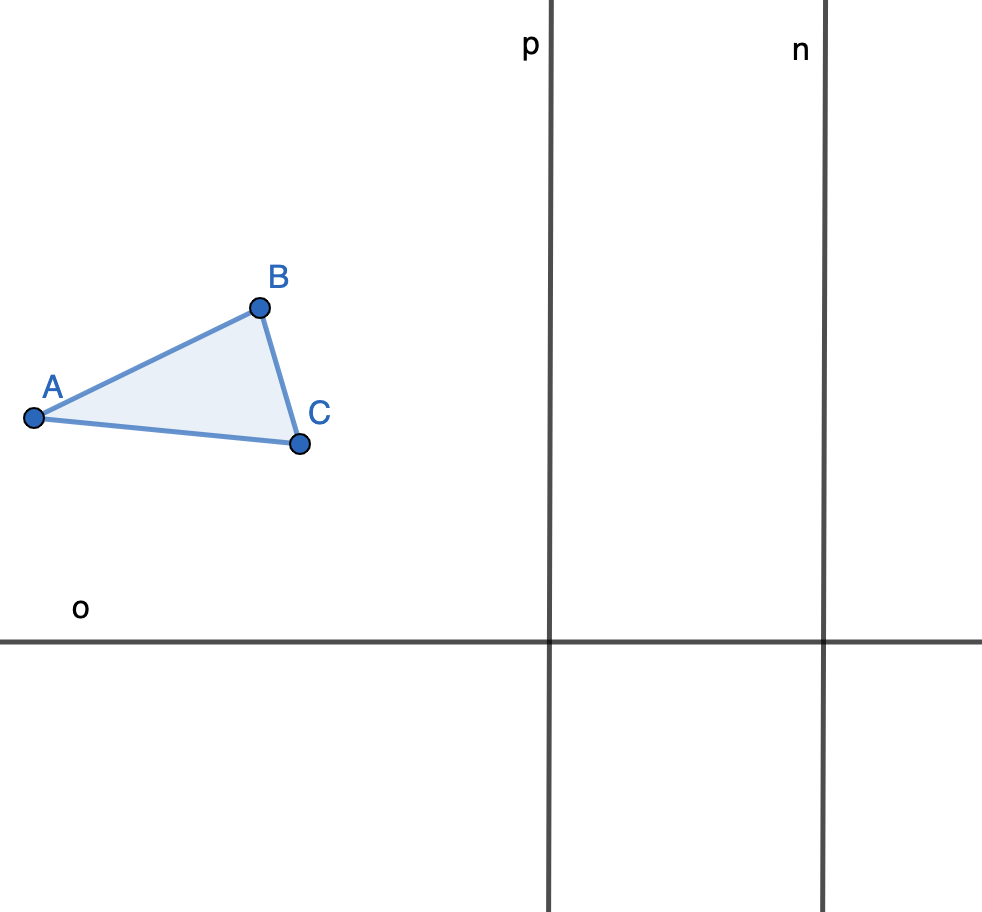
\includegraphics[height=0.45\textheight]{figure_6.png} 
	\end{center}
	
	
\end{enumerate}



\end{document}

\noindent Approved by the MDCC, .

\noindent Approved by the department of mathematics, .


